\chapter{Theoretical Background}

\section{Cloud Computing}
Cloud computing refers to the hardware, systems software, and applications delivered as services over the Internet \cite{cloud}. Cloud computing have services from a simple web services to data centers. Hardware for cloud computing can to consist of thousands of individual \emph{computing nodes} with their corresponding networking and storage subsystems, power distribution and conditioning equipment, and extensive cooling systems. Software for cloud computing can to consist of operative system in virtual machines, web applications and web services. 

Cloud computing have three deployment models: \emph{public, private} and \emph{hybrid}, and cloud services models can be grouped three categories:
\begin{itemize}
  \item Infraestructure as a Service(IaaS): providers offer computer power and   storage such as processors, virtual machines, data centers, serves, among others.
  \item Platform as a service(PaaS): providers offer the tools for developing applications such as operative systems, programming languages environments, databases among others.
  \item Software as a Service(SaaS): providers offer access to applications and databases.
\end{itemize}  

Figure \ref{cloud_services} show the stack estructure for cloud services.

\begin{figure}[!h]
\centering
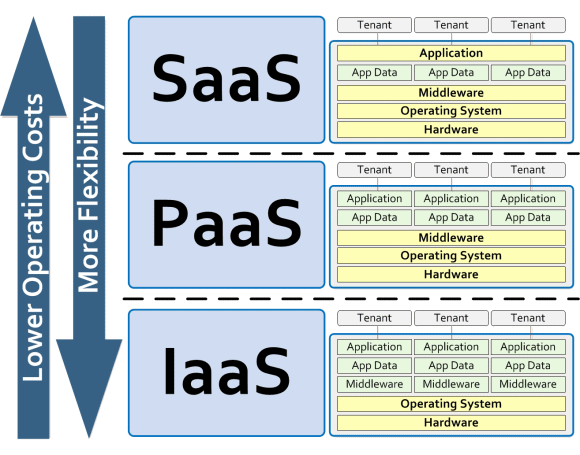
\includegraphics[width=0.5\textwidth]{images/cloud_services}
\caption[Cloud computing service models]{Cloud computing service models \\
\scriptsize{\textbf{Source:} \url{http://www.ibm.com/developerworks/websphere/techjournal/1206_dejesus/1206_dejesus.html}}}
\label{cloud_services}
\end{figure}

\subsection{Virtualisation}

Virtualisation are a important component for cloud computing to decoupled the operative system of the physical infrastructure for adding flexibility. Virtualisation allows rapid deployment, reduce space and energy costs thanks to in a server can be running multiple operative systems. The main aim of virtualisation technologies 
is to hide the physical characteristics of computing resources from the way in which other systems, applications, or end users interact with those resources \cite{virtualization}. Hardware platform, operative system, networks and storage devices can be virtualised. 

\subsubsection{Virtual Machines}
A Virtual Machine(VM) is an instance of the physical machine and gave users the illusion of accessing the physical machine directly \cite{virtualization}. VMs are created and executed in a host machine by Virtual Machine Monitor or Hypervisor. The VMs can run legacy applications requiring an older platform and/or OS and run isolated of the underlying system. Also, it can create a single system image starting from an heterogeneous collection of machines, and can be performed faster job migration within different virtual machines running on the same hardware. These characteristics have led to the use of virtual machines for cloud computing. 

\subsubsection{Network Function Virtualisation}
The Network Function Virtualisation(NFV) involves the implementation of network functions in software that can run on a range of industry standard server hardware, and that can be moved to, or instantiated in, various locations in the network as required, without the need for installation of new equipment \cite{nfv}. European Telecommunications Standards Institute (ETSI) define a NFV framework \cite{nfv_framework} with three main working domains like is showed in figure \ref{nfv_framework}. 


\begin{figure}[!h]
\centering
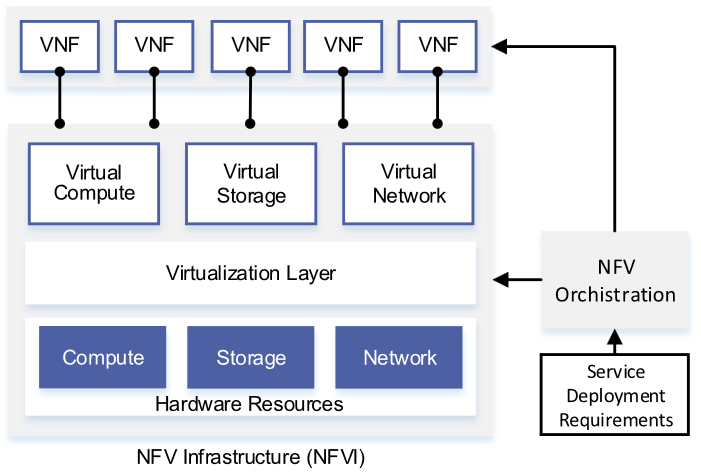
\includegraphics[width=0.5\textwidth]{images/nfv_framework}
\caption[Network Function Virtualisation Framework]{Network Function Virtualisation Framework \\
\scriptsize{\textbf{Source:} Software-Defined Network Function
Virtualisation: A Survey - Figure 1}}
\label{nfv_framework}
\end{figure}

The \emph{Virtualised Network Functions} (VNF) are the software implementation of a network function, \emph{NFV Infrastructure} (NFVI) including the diversity of physical resources and \emph{NFV Management and Orchestration} which covers the orchestration and life-cycle management of physical.
and/or software resources 

\subsubsection{Software-defined Network} 
Software-defined Networking (SDN) is a paradigm where a central software program, called a controller, dictates the overall network behavior\cite{sdn}. Basically, it separates vertical integration between the \emph{data plane} (networks control logic) and the \emph{control plane} (routers and switches). A \emph{logically centralized software program}   (or network operative system) implements the logic control of the network, and switches and routers become  simple forwarding devices. The figure \ref{sdn} shows the SDN architecture.

\begin{figure}[!h]
\centering
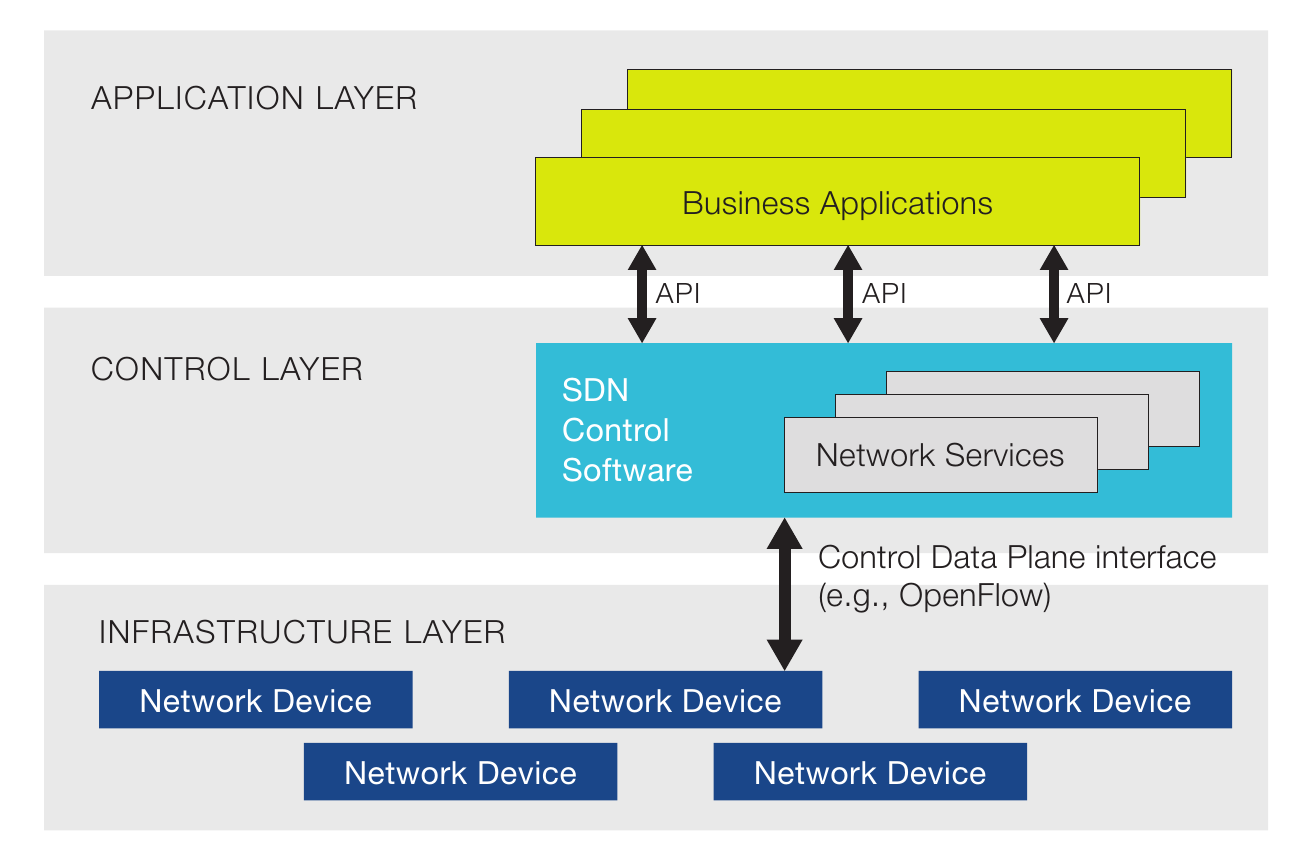
\includegraphics[width=0.5\textwidth]{images/sdn_architecture}
\caption[Software-define Networking]{Software-define Networking \\
\scriptsize{\textbf{Source:} \url{https://www.sdxcentral.com/resources/sdn/inside-sdn-architecture/}}}
\label{sdn}
\end{figure}

\section{Fog Computing}
Fog computing, also termed \emph{edge computing}, is considered a an extension of the cloud computing paradigm and it is a proposed paradigm to enable computing directly at the edge of the network \cite{fog}. This paradigm is a highly virtualised platform that provides compute, storage, and networking services without going to the cloud. The devices that are part of the fog computing infrastructure are called \emph{fog nodes} and they provide resources for services at the edge of the network. Fog nodes can be set-top-boxes, access points, routers, switches, base stations and end devices. They are interconnected and and each of them
is linked to the cloud. The figure \ref{fog} shows the fog computing architecture. In this figure can be observed that fog computing between the core and the edge of the network.

\begin{figure}[!h]
\centering
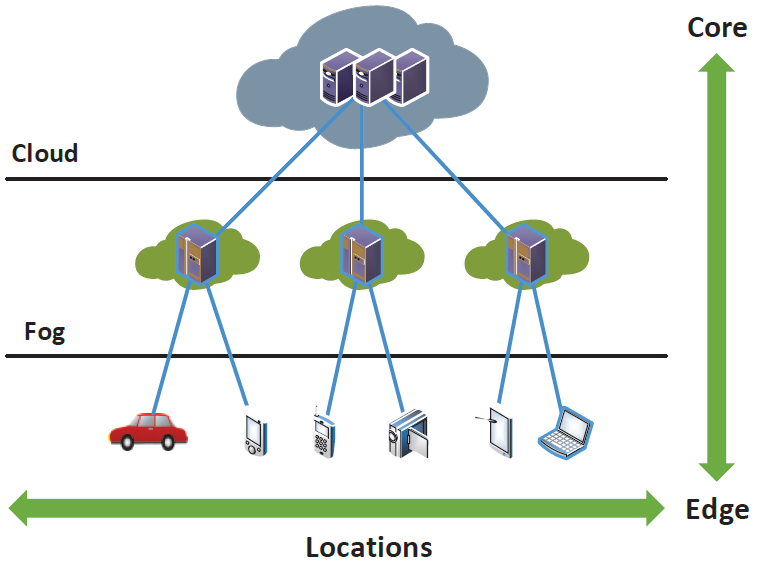
\includegraphics[width=0.5\textwidth]{images/fog}
\caption[Fog Computing Paradigm]{Fog Computing Paradigm \\
\scriptsize{\textbf{Source:} The Fog Computing Paradigm Scenarios and Security Issues - Figure 1}}
\label{fog}
\end{figure}

Fog computing includes the same services offered by cloud computing but closer to the end user and so provides low latency, location awareness, and improves quality-of-services (QoS) for streaming and real time applications like video streaming.

\section{Video Coding}
A problem of uncompressed video (RAW) files have been storage and transmission due to large number of bits containing, for this reason is required the use of compression techniques for reduce the bits number to represent a video. Video coding take advantage of elimination of three types of redundancy \cite{motion}:
\begin{itemize}
	\item Statistical redundancy: refers to the spatial correlation between neighbour pixels in a frame and temporal correlation between co-localisated pixel in consecutive frames.
	\item Psychovisual redundancy: is due to limitations and characteristics of human system visual that not distinguish certain information.
	\item Coding redundancy: is produced by the repetition of symbols representing video information.
\end{itemize}
	
The figure \ref{codec} depicts a blocks diagram of a standard \emph{video codec}. Generally, a video codec have  two main modules, the encoder and decoder. They uses techniques and tools exploit the redundancies aforementioned. 

\begin{figure}[!h]
\centering
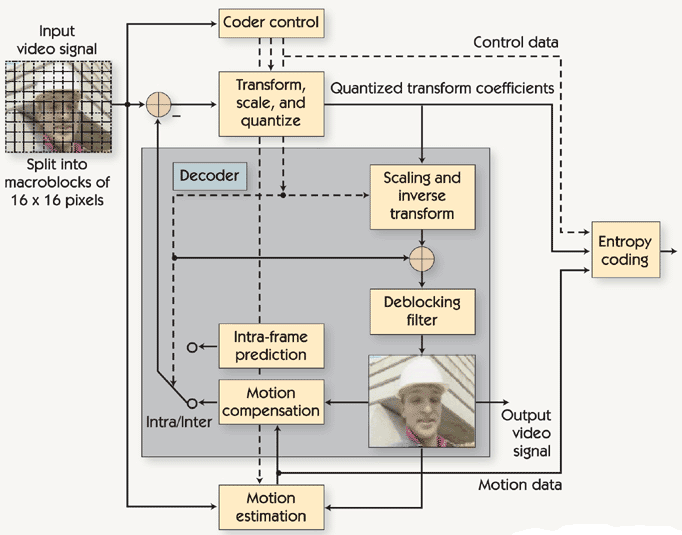
\includegraphics[width=0.6\textwidth]{images/codec}
\caption[Block Diagram of Video Codec]{Block Diagram of Video Codec \\
\scriptsize{\textbf{Source:} \url{http://www.eetimes.com/document.asp?doc_id=1272639}}}
\label{codec}
\end{figure}

Video encoder consist of three elements:
\begin{itemize}
	\item The predictor consists of intra-frame prediction for exploiting the spatial correlation. Also it consists of motion estimation and motion compensation for exploiting the temporal correlation. 
	\item The quantizer reduces the accuracy of the representations of the predictor by a fidelity criterion to eliminate the psychovisual redundancy.
	\item The entropy coding reduces the numbers of symbols necessary for representing the video.
\end{itemize}

Video decoder performs the inverse process of each elements to reconstruct the encoded information. In reconstruction process is presented information losses due to elimination or transformation of original information in the encoder.

\section{Compressive Sensing}

Lossy compression are used two assumptions: first is related to imperfection of human perception(sense) and the second related to the specific properties of signals in a certain transform domain. The aim of compressive sensing is to reconstruct a signal using a small set of signal samples \cite{compressive}. One of the main requirements that should be satisfied in order to efficiently apply the compressive sensing is the \emph{Sparsity}.

\subsection{Sparsity}

Consider a vector or signal $\boldsymbol{x} \in \mathbb{R}^N$ space. Given an orthonormal basis matrix (dictionary) $\boldsymbol{B} \in \mathbb{R}^{N \times N}$ whose columns are the basis elements $ \{\boldsymbol{b}_i\}_{i=1}^N$, $\boldsymbol{x}$ can be represented in terms of this basis as:
\begin{center}
\begin{equation}
\boldsymbol{x}=\sum \limits_{i=1}^{N} \alpha_i \boldsymbol{b}_i
\end{equation}
\end{center}
where $\boldsymbol{\alpha}$ is a vector of coefficients \cite{sparsity} and $\boldsymbol{b}_i$ are called \emph{atoms of a dictionary}. These coefficients are given by $\alpha_i = \boldsymbol{x} \boldsymbol{b}_i^T$. If the number of non-zero coefficients in $\boldsymbol{x}$ is $K\ll N$, the basis $\boldsymbol{b}$ provides a K-sparse representation of $\boldsymbol{x}$. Sparsity of vector $\boldsymbol{\alpha}$ is related
to $||\alpha||_0 = K$ where $||.||_p$ indicates the $\ell_p$-norm define as
\begin{equation}
||\boldsymbol{\alpha}||_p = \left(\sum\limits_{i=1}^{n} |\alpha_i|^p \right)^\frac{1}{p}
\end{equation}
and $||\alpha$ is the $\ell_0$-norm, which means the number of the non-zero elements of vector, and is defined  as
\begin{equation}
||\boldsymbol{\alpha}||_0 = \lim_{p \to 0} ||\alpha||_p^p=\lim_{p \to 0} \sum_i |\alpha_i|^p
\end{equation} 

Typically, real-world signals are not exactly sparse in any orthogonal basis. Instead, they are \emph{compressible}. A signal is compressible if its coefficient magnitudes, sorted in decreasing order, present a power law decay
\begin{equation}
|\alpha|_{(n)} \leq C n^{-s}\;,\quad s=1,2 \ldots
\end{equation}

where $|\alpha|_{(n)}$ is the nth largest entry of $\alpha$ and $C$ is a constant. Because the coefficients magnitudes decay so rapidly, a small number of vectors $K \ll N$ from $\boldsymbol{B}$ can provide accurate
approximations to $\boldsymbol{x}$. The error between original signal and its approximation is given by
\begin{equation}
||\boldsymbol{x}_L - \boldsymbol{x}||_2 \leq CL^{-(s-\frac{1}{2})}
\end{equation}
where $L$ is the $L$-term linear combination of elements that best approximate $\boldsymbol{x}$.  

\subsection{Incoherence Sampling}

A set of random measurements are selected from the signal $\boldsymbol{x}$ is used to construct $M \times N$ matrix $\boldsymbol{\phi}$ such as
\begin{equation}
\boldsymbol{y} = \boldsymbol{\phi x}
\end{equation}
where $\boldsymbol{y}$ is a $M\times 1$ vector of the compressive measurements. For reconstruct $\boldsymbol{x}$ from $\boldsymbol{y}$, $\boldsymbol{x}$ should be sparse in the transform domain (defined by the orthogonal basis matrix $\boldsymbol{B}$), such as
\begin{equation}
\boldsymbol{y}=\boldsymbol{\phi B \alpha}= \boldsymbol{D\alpha}
\end{equation}
Incoherence is related to the property that signals having sparse representation in the transform domain $\psi$ should be dense in the domain where the acquisition is performed \cite{compressive}. The coherence between sensing basis $\boldsymbol{\phi}$ and the representation basis $\boldsymbol{\psi}$ is given by
\begin{equation}
\mu(\boldsymbol{phi},\boldsymbol{B})= \sqrt{N} \max_{1 \leq j, j \leq N} | \boldsymbol{\varphi}_i,\boldsymbol{b}_j|, \quad 1\leq \mu(\boldsymbol{phi},\boldsymbol{B}) \sqrt{N}
\end{equation}
If the coherence is low, a number of random measurements to reconstruct the signal is small because each row of $\boldsymbol{phi}$ is spread out in the $\boldsymbol{B}$ domain.

\subsection{Restricted Isometric Property (RIP)}

This property helps to determine if matrix $\boldsymbol{D}$ is good for compressed sensing. A matrix $boldsymbol{D}$ satisfy the RIP if for each $K = 1,2, \ldots,$ the isometric constant $\delta_K$ of the matrix $\boldsymbol{D}$ is the smallest number such as
\begin{equation}
(1-\delta_K)||\boldsymbol{x}||_2^2 \leq ||\boldsymbol{Dx}||^2_2 \leq (1+\delta_K)||\boldsymbol{x}||^2_2
\end{equation}
holds for all K-sparse vectors $\boldsymbol{x}$. This property is equivalent to said that all subsets of $K$ columns taken from $\boldsymbol{D}$ are nearly orthogonal and K-sparse vectors cannot be in the null space
of $\boldsymbol{D}$.

\subsection{Numerical Optimisations}

$M \times N$ matrix represents a undetermined system of equations that can be have infinite solutions. The method to solve this system is to find the minimum-norm solution for the optimisation problem 
\begin{equation}
\min||\boldsymbol{\alpha^\prime}||_0 \quad \textrm{subject to} \; \boldsymbol{x} = \boldsymbol{D \alpha^\prime}
\end{equation}
Although this problem recover directly the K sparse signal, it is a NP-Hard problem because require a exhaustive combinatorial search. Instead, is used the $\ell_1$ and $\ell_2$-norm to approximate the sparse solution. The $\ell_1$-norm minimisation problem is given by
\begin{equation}
\min||\boldsymbol{\alpha^\prime}||_1 \quad \textrm{subject to}; \boldsymbol{x} = \boldsymbol{D \alpha^\prime}
\end{equation}
This norm is convex and in some cases yields the same results of $\ell_0$-norm minimisation.
\begin{equation}
\min||\boldsymbol{\alpha^\prime}||_1 \quad \textrm{subject to}; \boldsymbol{x} = \boldsymbol{D \alpha^\prime}
\end{equation}

Figure \ref{fig:compressive} summarise the process to obtain a compressible signal.
\begin{figure}[!h]
\centering
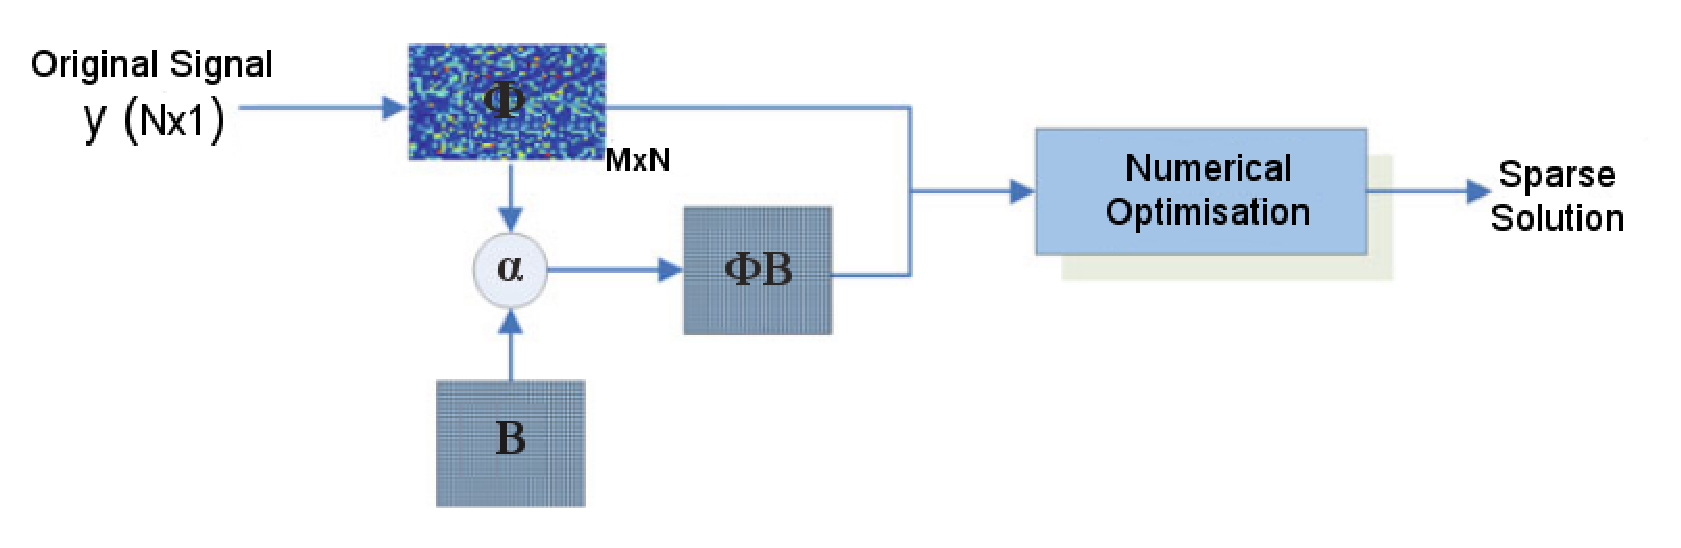
\includegraphics[width=\textwidth]{images/sparse.eps}
\caption[Compressive sensing procedure]{Compressive sensing procedure \cite{compressive}}
\label{fig:compressive}
\end{figure}


\subsection{Dictionaries}

For sparse representation the dictionary $B$ can be a predetermined matrix but, to have a better representation, the dictionary should be trained directly from the data. 








